%%%%%%%%%%%%%%%%%%%%%%%%%%%%%%%%%%%%%%%%%%%%%%%%%%%%%%%%%%%%%%%%%%%%%%%%%%%
\chapter{Étude de la viabilité technique}
\label{Chapitre_4}
%%%%%%%%%%%%%%%%%%%%%%%%%%%%%%%%%%%%%%%%%%%%%%%%%%%%%%%%%%%%%%%%%%%%%%%%%%%
\section{Introduction}
\label{sec:intro_chap4}
%%%%%%%%%%%%%%%%%%%%%%%%%%%%%%%%%%%%%%%%%%%%%%%%%%%%%%%%%%%%%%%%%%%%%%%%%%%

Les chapitres précédents ont établi que Vocallia répond à un besoin structurel, sur un marché captif, selon un modèle économique scalable et défendable. Ces conclusions ne valent toutefois qu'à une condition sine qua non~: que la solution soit techniquement réalisable, opérationnellement fiable et industriellement déployable avec les technologies disponibles aujourd'hui. Une infrastructure conversationnelle vocale en dialecte tunisien, capable de soutenir des appels sortants en temps quasi réel, avec une qualité dialectale suffisante pour ne pas dégrader l'expérience client, ne se résume pas à un assemblage d'API~: elle exige une orchestration rigoureuse, une gestion fine de la latence, une résilience face aux défaillances de fournisseurs tiers et une conformité réglementaire intégrée dès la conception.

Ce chapitre démontre, étape par étape, que cette exigence peut être tenue. L'analyse procède par couches successives~: des exigences fonctionnelles et non fonctionnelles à l'architecture globale, puis aux modules logiques, au pipeline conversationnel et à l'orchestration IA, jusqu'aux dimensions transverses que sont la sécurité, la scalabilité, l'observabilité et le déploiement. Chaque décision technique est justifiée par les objectifs produit définis aux chapitres~2 et~3~: maîtrise du darija, soutenabilité du coût par appel, fiabilité opérationnelle, traçabilité complète et conformité INPDP. Le chapitre se conclut par l'examen lucide des limites techniques résiduelles et des mécanismes de mitigation associés. L'objectif n'est pas de décrire une stack — c'est de prouver que l'architecture choisie rend Vocallia non seulement faisable, mais durablement opérable et évolutive.

%%%%%%%%%%%%%%%%%%%%%%%%%%%%%%%%%%%%%%%%%%%%%%%%%%%%%%%%%%%%%%%%%%%%%%%%%%%
\section{Exigences et contraintes techniques}
\label{sec:exigences_techniques}
%%%%%%%%%%%%%%%%%%%%%%%%%%%%%%%%%%%%%%%%%%%%%%%%%%%%%%%%%%%%%%%%%%%%%%%%%%%

La définition rigoureuse des exigences techniques est la condition initiale de toute architecture cohérente. Trois familles d'exigences structurent la conception de Vocallia~: les exigences fonctionnelles, qui décrivent ce que le système doit faire~; les exigences non fonctionnelles, qui définissent comment il doit le faire~; et les contraintes spécifiques au projet, qui bornent l'espace des solutions techniquement et réglementairement acceptables.

\subsection{Exigences fonctionnelles}
\label{subsec:exigences_fonctionnelles}

Les exigences fonctionnelles découlent directement du parcours client défini en section~3.7 et de la promesse produit formulée en section~3.2. Elles couvrent six familles de capacités. La première concerne la \textbf{gestion des organisations et des utilisateurs}~: création de comptes marchands, hiérarchie de rôles (administrateur, opérateur, lecture seule), invitation de collaborateurs, gestion d'équipes par organisation. La deuxième porte sur la \textbf{gestion des campagnes et des appels}~: réception des commandes via webhook, planification d'appels sortants, paramétrage de scripts par campagne, gestion des relances, file d'attente avec priorisation. La troisième regroupe les \textbf{capacités conversationnelles}~: reconnaissance vocale en darija avec code-switching arabe/français, compréhension d'intentions (confirmation, annulation, demande d'information, indisponibilité), génération de réponses naturelles, synthèse vocale en dialecte tunisien. La quatrième couvre les \textbf{intégrations métier}~: connecteurs natifs avec les principales plateformes e-commerce (Shopify, WooCommerce), API REST pour intégrations personnalisées, webhooks de remontée de statut. La cinquième concerne le \textbf{tableau de bord et le reporting}~: visualisation des appels en quasi-temps réel, métriques agrégées (taux de confirmation, taux de joignabilité, durée moyenne), export de transcriptions, rapports mensuels automatisés. La sixième porte sur l'\textbf{administration et l'observabilité}~: gestion des secrets API, supervision des intégrations, journaux d'audit, alerting opérationnel.

\subsection{Exigences non fonctionnelles}
\label{subsec:exigences_non_fonctionnelles}

Les exigences non fonctionnelles définissent les seuils de qualité opérationnelle que l'architecture vise à garantir. Elles sont synthétisées dans le tableau~\ref{tab:exigences_nf}~: chacune est posée comme un objectif technique réaliste, à atteindre par les choix d'architecture détaillés dans la suite du chapitre.

\begin{table}[H]
\centering
\caption{Exigences non fonctionnelles — cibles techniques de Vocallia}
\label{tab:exigences_nf}
\begin{tabular}{|p{4cm}|p{5cm}|p{5cm}|}
\hline
\textbf{Dimension} & \textbf{Cible technique} & \textbf{Justification produit} \\
\hline
Latence conversationnelle & Délai de réponse de bout en bout visé autour d'une seconde par tour de parole & Seuil au-delà duquel l'échange est perçu comme artificiel et dégrade l'expérience client \\
\hline
Disponibilité du service & Cible élevée, compatible avec un usage e-commerce continu & Limiter au strict minimum les fenêtres d'indisponibilité affectant la confirmation des commandes \\
\hline
Scalabilité horizontale & Capacité à absorber la croissance du volume d'appels sans refonte & Permet d'accompagner la trajectoire commerciale projetée jusqu'au scénario ambitieux d'année~3 \\
\hline
Sécurité des données & Chiffrement en transit (TLS) et au repos sur les données sensibles & Conformité INPDP et standards de sécurité B2B exigés par les clients institutionnels \\
\hline
Multi-tenancy & Isolation logique stricte entre organisations & Indispensable pour un SaaS B2B servant plusieurs marchands potentiellement concurrents \\
\hline
Observabilité & Couverture logs, métriques et traces & Diagnostic rapide des incidents et amélioration continue des performances dialectales \\
\hline
Évolutivité fonctionnelle & Architecture modulaire à couplage faible & Permet l'ajout de nouveaux cas d'usage (relance, prise de RDV) sans refonte \\
\hline
\end{tabular}
\end{table}

\subsection{Contraintes spécifiques au projet}
\label{subsec:contraintes_projet}

Au-delà des exigences génériques d'un SaaS B2B, Vocallia opère sous quatre contraintes spécifiques qui ont guidé l'ensemble des choix architecturaux. La \textbf{contrainte linguistique} est la plus structurante~: aucun fournisseur d'API global ne maîtrise nativement le darija avec son code-switching arabe/français caractéristique. L'architecture doit donc intégrer des couches d'adaptation propriétaires (ingénierie de prompts, normalisation phonétique, post-traitement) sur des modèles génériques. La \textbf{contrainte réglementaire} impose une conformité ab initio à la loi n°2004-63 et aux exigences de l'INPDP~: consentement explicite, durée de rétention bornée à 30~jours, droit de suppression, traçabilité des traitements. La \textbf{contrainte économique} découle directement du modèle de tarification présenté en section~3.8~: le coût variable par appel de deux minutes, estimé à environ 0{,}27~DT, doit rester compatible avec un prix d'entrée du palier Starter de 0{,}79~DT par appel, afin de préserver une marge brute soutenable de l'ordre de 65~\% sur ce palier. La \textbf{contrainte de dépendance fournisseurs}, enfin, impose une architecture multi-fournisseurs ouvrant la possibilité de substituer un provider STT, LLM, TTS ou téléphonie en cas de hausse tarifaire ou d'interruption — exigence directement issue de l'analyse SWOT en section~3.4.

\begin{quote}
\textbf{Lecture stratégique des exigences.} Les quatre contraintes spécifiques agissent comme un \emph{filtre architectural}~: chaque décision technique du présent chapitre est évaluée à l'aune de sa capacité à respecter simultanément la cible de latence, la soutenabilité économique du plan Starter, la conformité INPDP et la substituabilité des fournisseurs. Une solution qui satisferait trois de ces quatre critères mais en échouerait un seul est rejetée. Cette discipline distingue une architecture viable d'un assemblage opportuniste de technologies.
\end{quote}

%%%%%%%%%%%%%%%%%%%%%%%%%%%%%%%%%%%%%%%%%%%%%%%%%%%%%%%%%%%%%%%%%%%%%%%%%%%
\section{Architecture technique globale}
\label{sec:architecture_globale}
%%%%%%%%%%%%%%%%%%%%%%%%%%%%%%%%%%%%%%%%%%%%%%%%%%%%%%%%%%%%%%%%%%%%%%%%%%%

L'architecture globale de Vocallia adopte un modèle en couches à responsabilités séparées, conçu pour maximiser la modularité, la testabilité et la substituabilité des composants externes. Cinq couches structurent le système, organisées de l'interface utilisateur jusqu'aux services tiers. La figure~\ref{fig:architecture_globale} en donne une vue synthétique~; les sous-sections qui suivent en commentent les choix les plus structurants.

\begin{figure}[H]
\centering
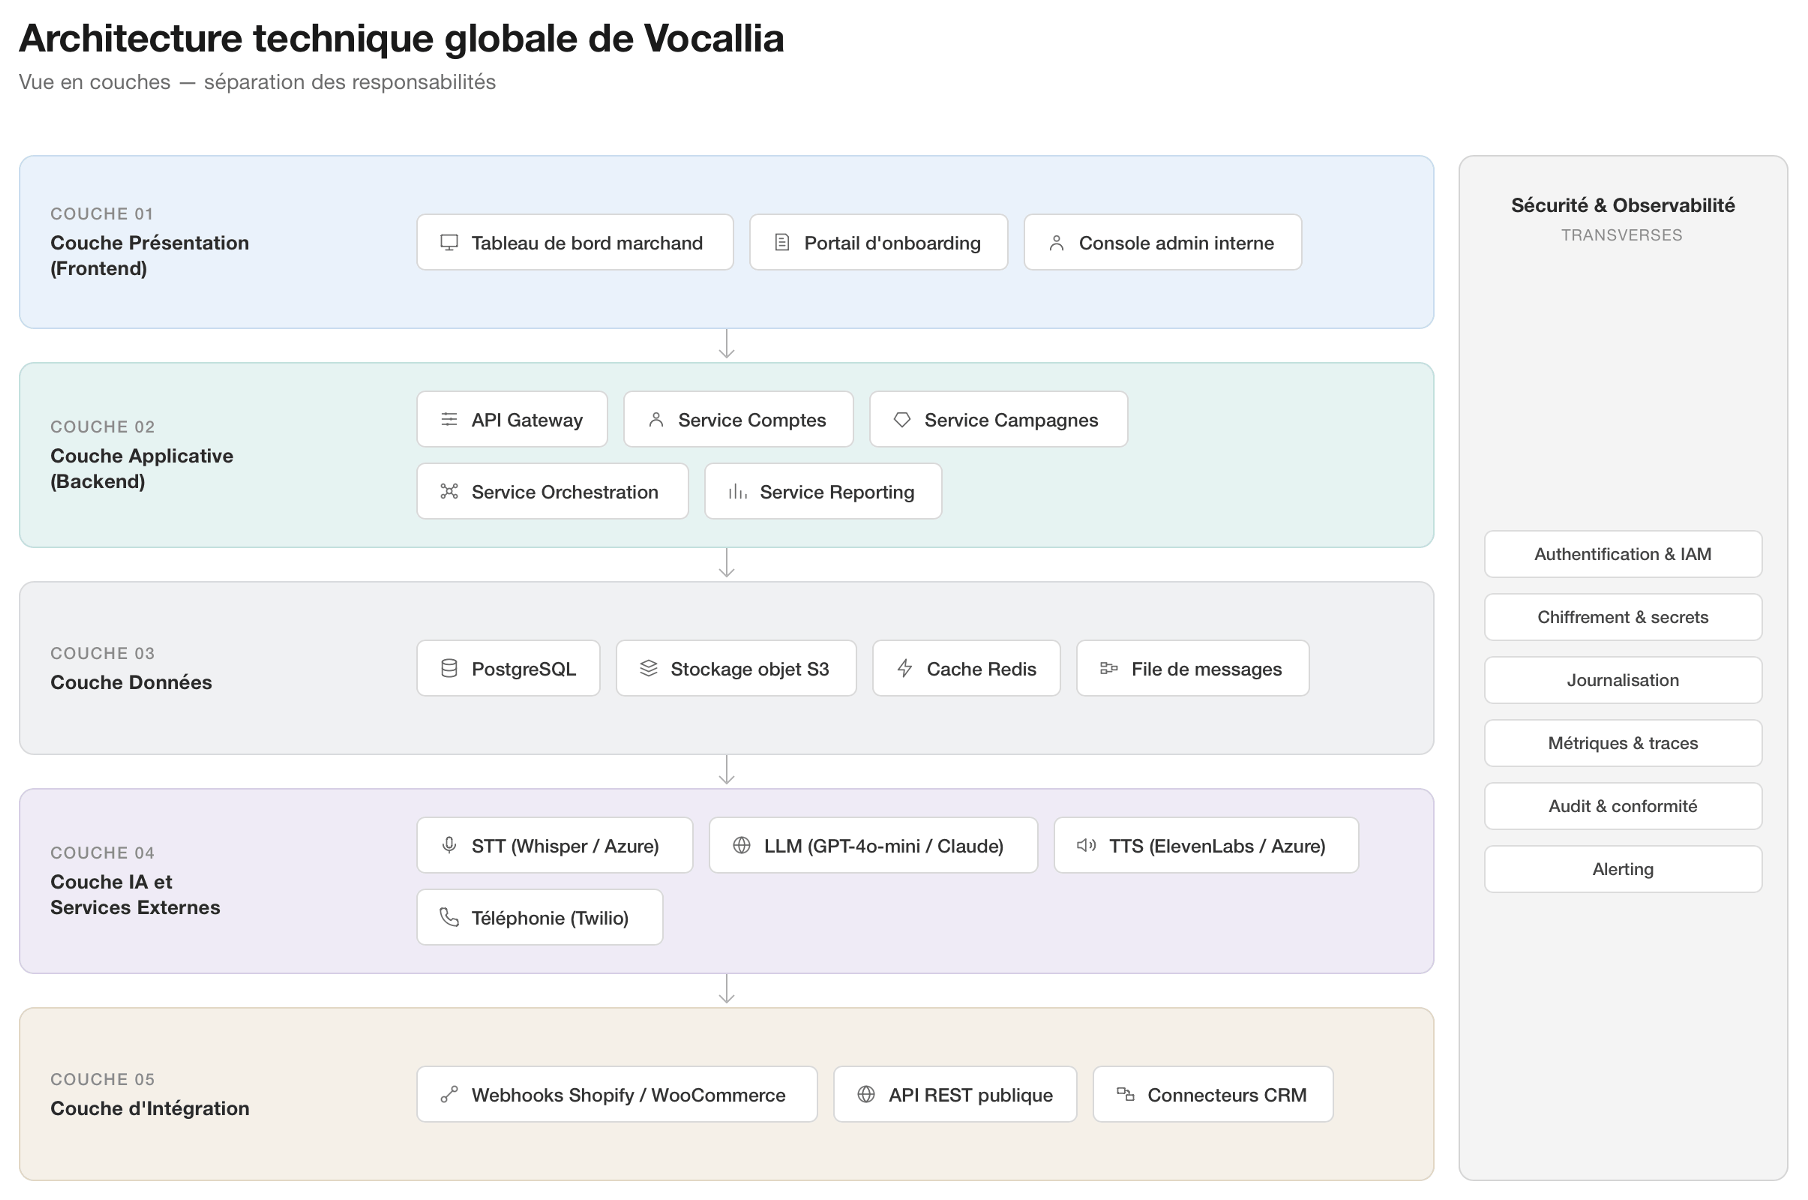
\includegraphics[width=\textwidth]{figures/architecture_globale_vocallia.png}
\caption{Architecture technique globale de Vocallia — vue en couches}
\label{fig:architecture_globale}
\end{figure}

\subsection{Couche présentation}
\label{subsec:couche_frontend}

La couche présentation regroupe les interfaces utilisateur destinées aux marchands et aux administrateurs~: tableau de bord web responsive, portail d'onboarding self-service et console interne de supervision. Elle communique exclusivement avec la couche applicative via une API REST sécurisée. Aucune logique métier ne réside côté client, ce qui garantit la portabilité future vers des applications mobiles ou des intégrations partenaires sans duplication de code critique.

\subsection{Couche applicative}
\label{subsec:couche_backend}

La couche applicative constitue le cœur fonctionnel du système. Elle est structurée autour d'une \textbf{API Gateway} centralisée qui authentifie, autorise et route les requêtes vers une constellation de services métier découplés~: gestion des comptes, gestion des campagnes, planification des appels, orchestration conversationnelle, reporting. Cette modularité autorise un déploiement et un dimensionnement indépendants de chaque service en fonction de sa charge réelle — l'orchestration conversationnelle, plus exigeante, étant scalée différemment du reporting, qui reste à charge faible et stable.

\subsection{Couche données}
\label{subsec:couche_donnees}

La couche données combine plusieurs typologies de stockage, chacune adaptée à sa fonction. Une \textbf{base de données relationnelle} (PostgreSQL) héberge les données transactionnelles structurées~: comptes, organisations, campagnes, statuts d'appels, transcriptions textuelles. Un \textbf{stockage objet} (compatible S3) abrite les enregistrements audio bruts, soumis à une politique de rétention de 30~jours par défaut. Un \textbf{cache distribué} (Redis ou équivalent) accélère les opérations à forte fréquence~: gestion de sessions, files d'attente, paramètres de configuration. Une \textbf{file de messages} (RabbitMQ, NATS ou équivalent) découple les déclencheurs d'appels du moteur d'exécution, permettant l'absorption de pics de charge sans dégradation perceptible côté marchand.

\subsection{Couche IA et services externes}
\label{subsec:couche_ia_externes}

La couche IA encapsule les appels aux fournisseurs externes derrière une interface d'abstraction unique. Trois familles de services sont mobilisées~: les \textbf{moteurs de reconnaissance vocale} (Whisper d'OpenAI à titre principal, avec adaptateurs vers Azure Speech ou Google Speech-to-Text en repli), les \textbf{modèles de langage} (GPT-4o-mini comme moteur de référence, avec adaptateurs vers Claude ou Mistral) et les \textbf{moteurs de synthèse vocale} (ElevenLabs en référence, avec Azure Neural TTS et Coqui en alternative). Cette abstraction est la traduction technique de l'exigence de substituabilité~: changer un fournisseur n'impacte qu'une classe d'adaptateur, jamais le code applicatif.

\subsection{Couche d'intégration}
\label{subsec:couche_integration}

La couche d'intégration assure les échanges bidirectionnels avec l'écosystème du marchand. Elle comprend des \textbf{connecteurs entrants} (webhooks Shopify, WooCommerce, API personnalisée pour systèmes propriétaires) qui déclenchent les campagnes d'appels, et des \textbf{connecteurs sortants} qui remontent les résultats vers le système du marchand (mise à jour de statut commande, alertes, synchronisation CRM). Le \textbf{module de téléphonie}, fondé sur Twilio à titre principal et conçu de manière abstraite pour permettre à terme un basculement vers un opérateur local, constitue l'interface critique vers le réseau téléphonique commuté.

\begin{quote}
\textbf{Cohérence architecture / objectifs produit.} Cette structure en cinq couches répond directement aux objectifs produit définis aux chapitres précédents. La séparation frontend / backend rend possible une distribution 100~\% digitale et un onboarding sans friction. La modularité des services applicatifs garantit l'évolutivité vers de nouveaux cas d'usage sans refonte. L'abstraction de la couche IA matérialise l'exigence de résilience multi-fournisseurs identifiée dans l'analyse SWOT. La couche d'intégration ouverte assure enfin la compatibilité avec l'écosystème e-commerce tunisien, condition d'adoption par des marchands déjà équipés.
\end{quote}

%%%%%%%%%%%%%%%%%%%%%%%%%%%%%%%%%%%%%%%%%%%%%%%%%%%%%%%%%%%%%%%%%%%%%%%%%%%
\section{Architecture logique et modulaire}
\label{sec:architecture_logique}
%%%%%%%%%%%%%%%%%%%%%%%%%%%%%%%%%%%%%%%%%%%%%%%%%%%%%%%%%%%%%%%%%%%%%%%%%%%

Là où l'architecture globale décrit la structure physique du système, l'architecture logique en décrit les responsabilités fonctionnelles. Vocallia est organisé en sept modules métier, conçus pour être faiblement couplés, indépendamment testables et évolutifs sans impact transversal. La figure~\ref{fig:architecture_logique} en propose la cartographie~; les sous-sections qui suivent ne reprennent pas exhaustivement chaque module, mais en précisent le rôle dans l'économie générale du système.

\begin{figure}[H]
\centering
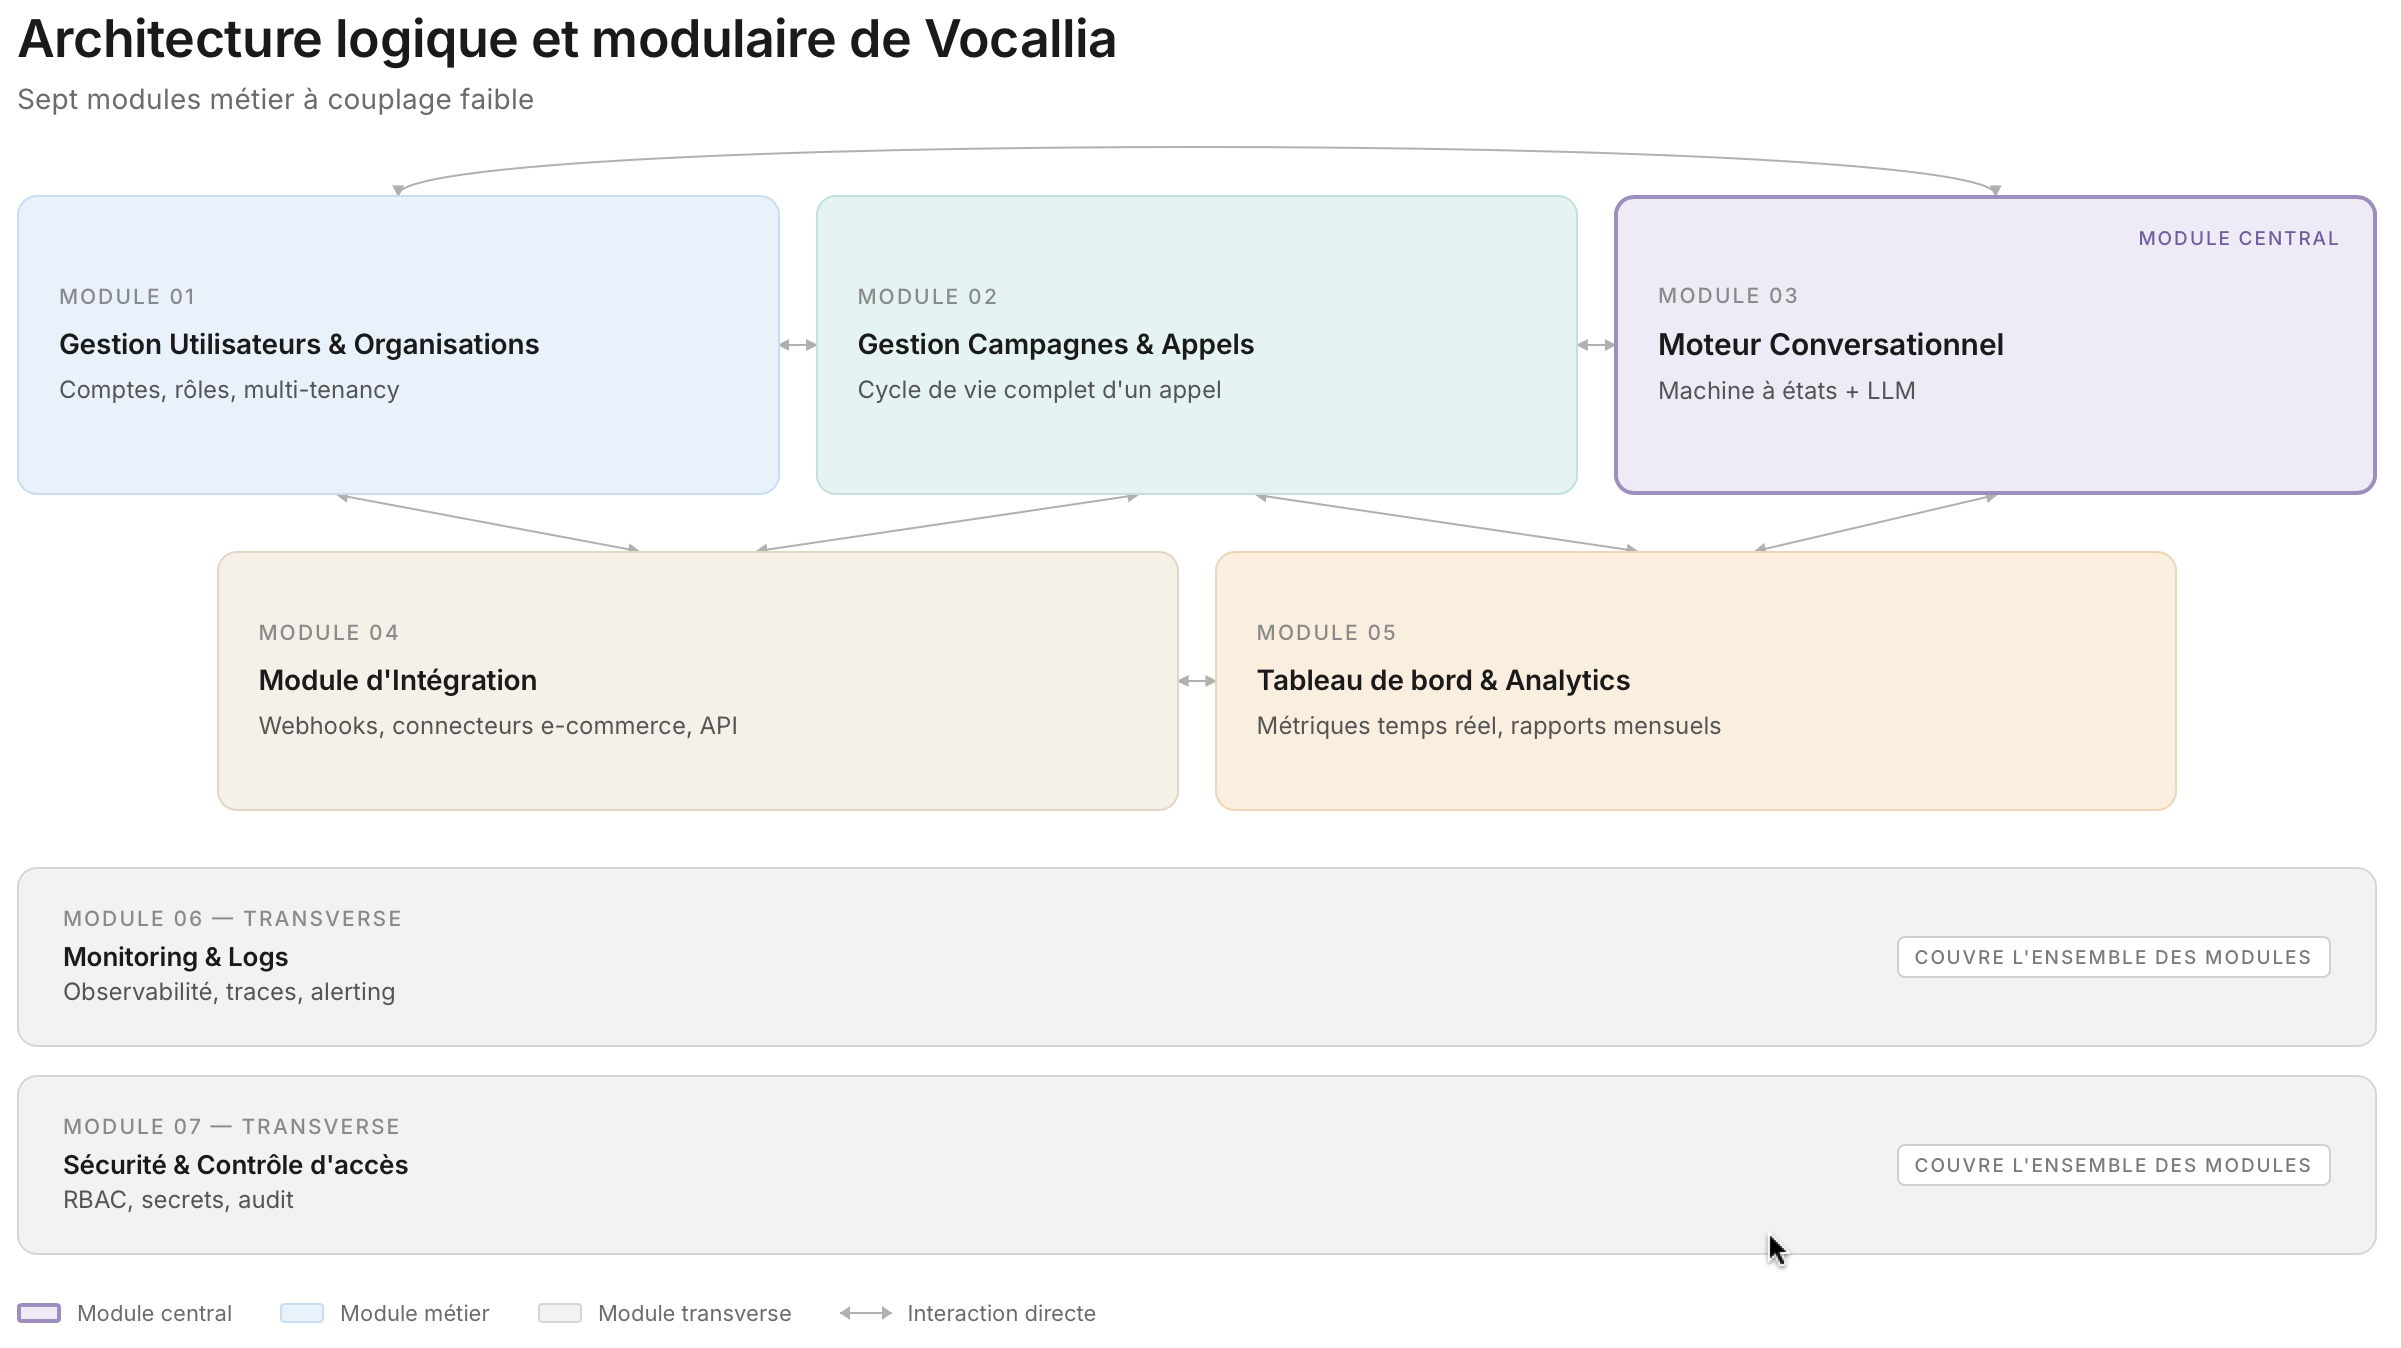
\includegraphics[width=\textwidth]{figures/architecture_logique_vocallia.png}
\caption{Architecture logique et modulaire de Vocallia — sept modules métier}
\label{fig:architecture_logique}
\end{figure}

\subsection{Modules d'identité et de campagnes}
\label{subsec:modules_id_campaigns}

Le module de \textbf{gestion des utilisateurs et des organisations} encapsule les opérations relatives à l'identité et constitue le socle de la multi-tenancy~: chaque ressource créée ailleurs est rattachée à une organisation, qui sert de frontière logique d'isolation pour toutes les requêtes ultérieures. Le module de \textbf{gestion des campagnes et des appels} orchestre le cycle de vie complet d'un appel — de la réception du webhook à la classification du résultat — et intègre la logique de relance automatique selon une stratégie d'intervalles configurable.

\subsection{Module moteur conversationnel}
\label{subsec:module_conversational}

Le moteur conversationnel est le composant le plus critique de l'architecture. Il implémente la machine à états du dialogue~: à chaque tour de parole, il reçoit la transcription du client, détermine l'intention, sélectionne la prochaine action et génère la réponse vocale. Sa structuration interne combine une couche déterministe (machine à états et règles métier) et une couche probabiliste (LLM pour l'interprétation des énoncés ambigus). Cette double nature, détaillée en section~\ref{sec:orchestration_ia}, garantit la prédictibilité du comportement sur les chemins critiques tout en préservant la souplesse conversationnelle attendue d'un agent vocal.

\subsection{Modules d'intégration, de tableau de bord et de monitoring}
\label{subsec:modules_horizontaux}

Le module d'\textbf{intégration} centralise les connexions aux systèmes externes du marchand~: gestion des webhooks entrants et sortants, transformations de format, gestion des erreurs (retry, dead-letter queue, alerting). Une bibliothèque de connecteurs natifs couvre les plateformes les plus courantes, tandis qu'une API générique permet l'intégration avec tout système exposant un endpoint REST. Le module de \textbf{tableau de bord et analytics} agrège, transforme et restitue les données opérationnelles aux marchands en quasi-temps réel, et alimente le rapport mensuel automatique présenté comme \emph{preuve physique} en section~3.6. Le module de \textbf{monitoring et logs}, transverse à l'ensemble du système, collecte logs, métriques et traces distribuées et déclenche les alertes pertinentes lorsque les seuils techniques sont franchis.

\subsection{Module de sécurité et contrôle d'accès}
\label{subsec:module_securite}

Le module de sécurité centralise les mécanismes transverses de protection~: gestion des tokens d'authentification, contrôle d'accès basé sur les rôles (RBAC), gestion des secrets API via un coffre-fort dédié, journalisation d'audit des actions sensibles et application des politiques de rétention. Sa conception isolée garantit que toute modification des règles de sécurité n'impacte qu'un point unique, réduisant le risque de configuration incohérente.

\begin{quote}
\textbf{Justification de la modularité.} Cette décomposition n'est pas un exercice théorique~: elle traduit en architecture la roadmap produit définie en section~3.6. L'extension future vers les cas d'usage de relance après abandon de panier, de prise de rendez-vous médicaux ou de qualification de leads ne nécessitera pas la création d'un nouveau système, mais l'instanciation de scénarios additionnels dans le moteur conversationnel et l'ajout de connecteurs dans le module d'intégration. Le socle technique est ainsi mutualisé entre tous les cas d'usage~: un seul corpus dialectal à enrichir, un seul tableau de bord à maintenir, une seule logique de sécurité à auditer. C'est cette mutualisation qui rend économiquement et techniquement crédible la transition d'un outil mono-usage vers une plateforme conversationnelle.
\end{quote}

%%%%%%%%%%%%%%%%%%%%%%%%%%%%%%%%%%%%%%%%%%%%%%%%%%%%%%%%%%%%%%%%%%%%%%%%%%%
\section{Pipeline conversationnel de Vocallia}
\label{sec:pipeline_conversationnel}
%%%%%%%%%%%%%%%%%%%%%%%%%%%%%%%%%%%%%%%%%%%%%%%%%%%%%%%%%%%%%%%%%%%%%%%%%%%

Le pipeline conversationnel est la séquence technique qui, à partir d'une commande reçue, produit un appel téléphonique automatisé en dialecte tunisien et restitue son résultat dans le système du marchand. Il constitue la chaîne de valeur technique de Vocallia~: chacun de ses maillons doit être individuellement performant, mais c'est l'orchestration de l'ensemble qui détermine la qualité perçue par le client final. La figure~\ref{fig:pipeline_conversationnel} en représente la séquence complète et le budget de latence cible. Les paragraphes qui suivent ne paraphrasent pas le schéma~: ils en explicitent les choix techniques les plus sensibles.

\begin{figure}[H]
\centering
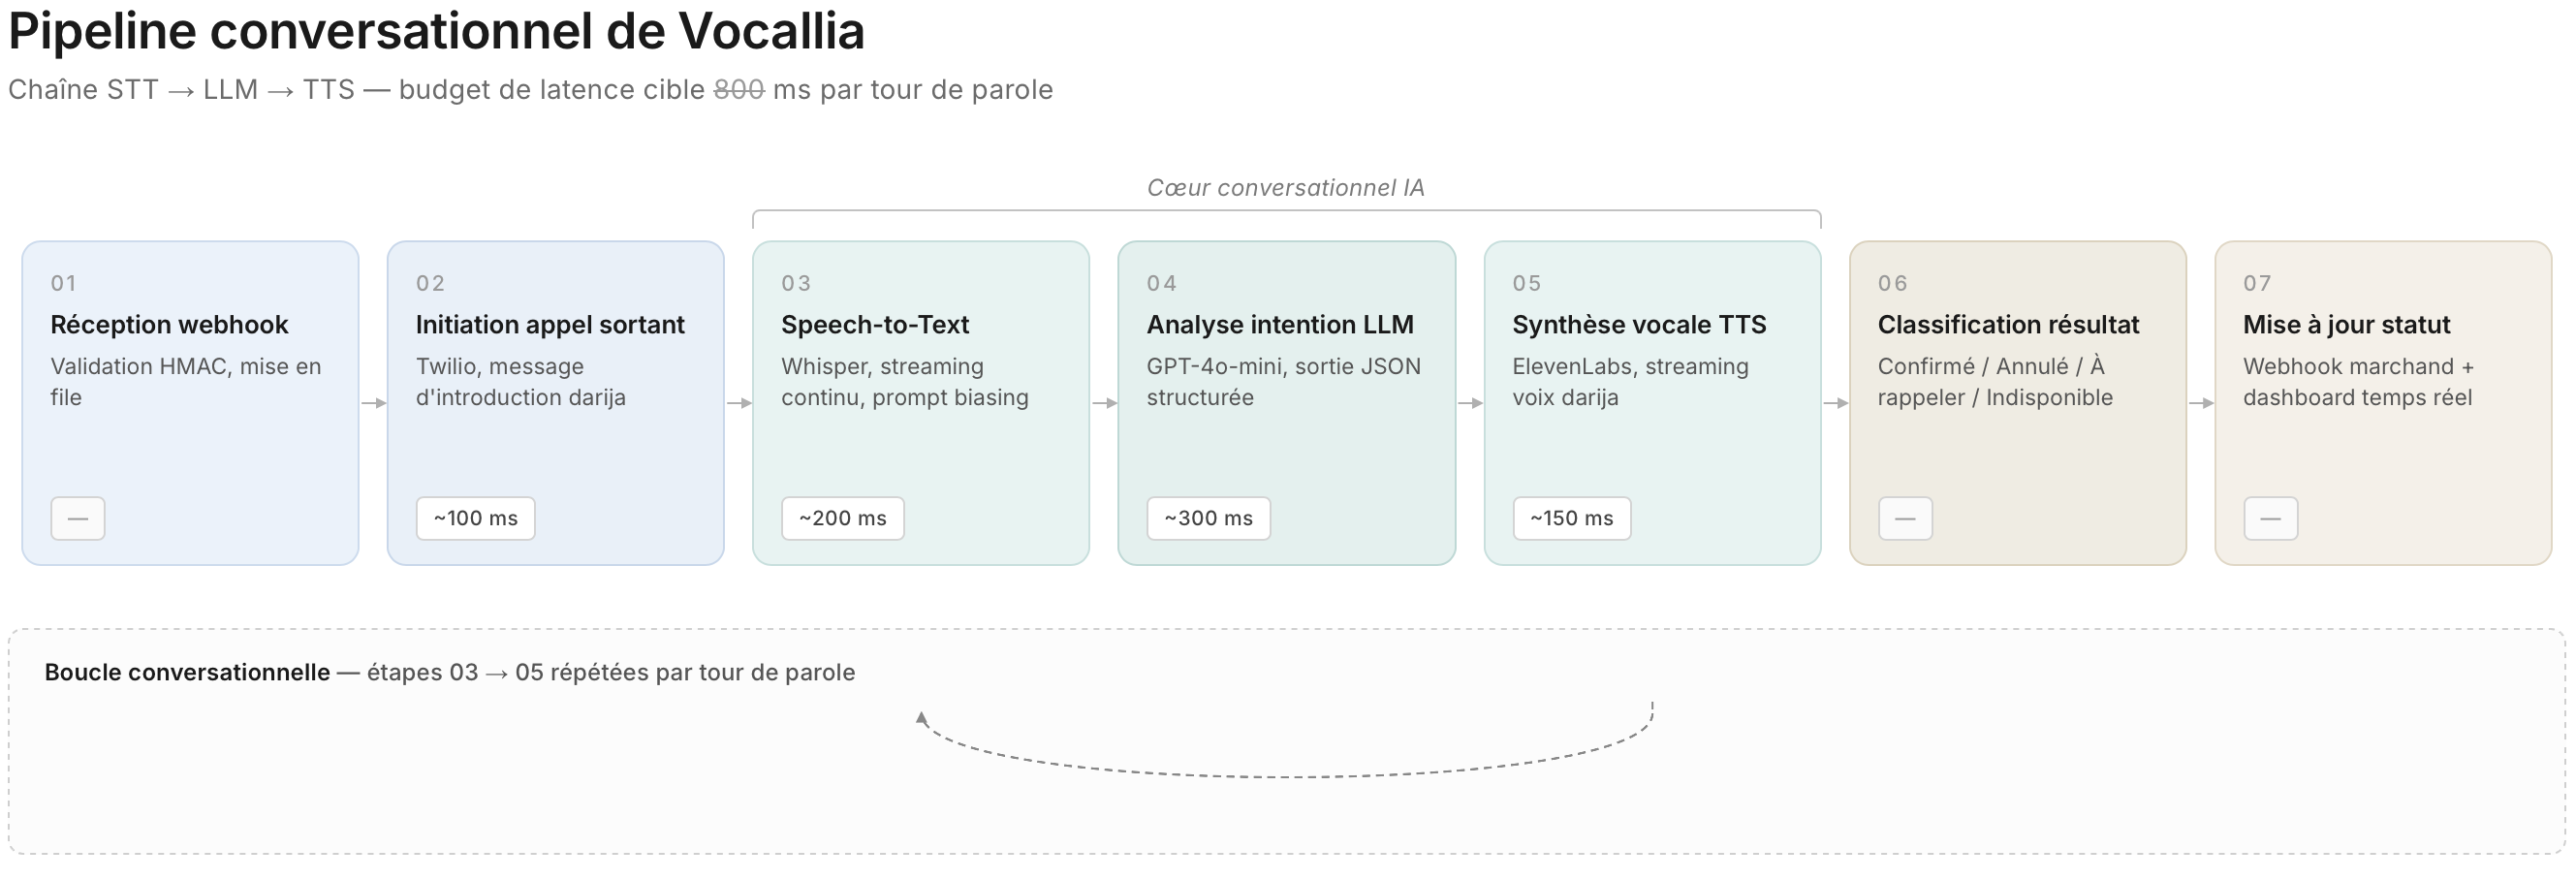
\includegraphics[width=\textwidth]{figures/pipeline_conversationnel_vocallia.png}
\caption{Pipeline conversationnel de Vocallia — chaîne STT $\to$ LLM $\to$ TTS et budget de latence}
\label{fig:pipeline_conversationnel}
\end{figure}

\subsection{Réception, déclenchement et message d'introduction}
\label{subsec:pipeline_amont}

À la réception d'une commande, un \textbf{webhook} est émis vers l'API de Vocallia. Le module d'intégration valide la signature (HMAC), authentifie l'organisation source, normalise les données et insère un job dans la file d'attente d'appels. Une réponse 200~OK est renvoyée immédiatement, garantissant que le webhook ne bloque pas le système du marchand même en cas de pic. Le worker d'exécution dépile ensuite le job, sélectionne la voix synthétique adaptée et déclenche l'appel sortant via l'API de téléphonie. Dès le décrochage, un \textbf{message d'introduction} en darija est diffusé pour signaler explicitement la nature automatisée de l'appel — exigence légale (loi n°2004-63) et bonne pratique conversationnelle qui réduit la confusion du destinataire.

\subsection{Reconnaissance vocale, analyse d'intention et synthèse vocale}
\label{subsec:pipeline_coeur}

Le flux audio du client est transmis au moteur STT en streaming continu. Whisper, principal moteur retenu, présente une couverture acceptable de l'arabe avec des limites documentées sur les sous-registres dialectaux les plus éloignés du standard. Vocallia compense ces limites par trois mécanismes complémentaires~: une \textbf{normalisation phonétique} en post-traitement, un \textbf{lexique de termes spécifiques} (noms de produits, vocabulaire e-commerce tunisien) injecté en \emph{prompt biasing} et un \textbf{score de confiance} évalué pour chaque énoncé. Lorsque la confiance descend sous un seuil défini, le moteur conversationnel déclenche une demande de clarification plutôt que d'inférer une intention non fiable.

Le texte transcrit est transmis au LLM avec un \textbf{prompt système} décrivant le contexte (commande, client, marchand), les intentions admises et les règles de réponse. Le modèle produit une sortie \textbf{structurée au format JSON} contenant l'intention détectée, les paramètres extraits, un score de confiance et une réponse textuelle. Cette structuration est délibérée~: elle permet d'appliquer des règles métier déterministes par-dessus la décision probabiliste du modèle, garantissant la prédictibilité sur les chemins critiques. La réponse est enfin transmise au TTS, configuré avec une voix adaptée au rendu darija. La synthèse fonctionne en \textbf{streaming bout en bout}~: l'audio est diffusé au client à mesure qu'il est généré, ce qui contracte significativement la latence perçue par rapport à une exécution séquentielle.

\subsection{Classification du résultat et restitution}
\label{subsec:pipeline_aval}

À l'issue de la conversation, le module de classification consolide les éléments collectés et attribue un résultat catégoriel à l'appel~: \emph{confirmé}, \emph{annulé}, \emph{à rappeler}, \emph{injoignable}, \emph{transféré à un humain} ou \emph{indéterminé}. Cette classification, qui combine intentions détectées et métadonnées techniques, est ensuite remontée en parallèle vers le \textbf{système du marchand} (mise à jour du statut de commande via webhook sortant) et vers le \textbf{tableau de bord} (mise à jour temps réel par WebSocket ou Server-Sent Events). La transcription complète et l'enregistrement audio sont stockés selon la politique de rétention configurée, et restent consultables par le marchand pour vérification ou ajustement des scripts.

\begin{quote}
\textbf{Budget de latence — analyse critique.} La cible globale d'environ une seconde par tour de parole est obtenue en allouant un budget par étape, indiqué sur la figure~\ref{fig:pipeline_conversationnel}. Cette répartition reste exigeante mais cohérente avec les performances publiées par les fournisseurs principaux. La marge de sécurité repose sur trois leviers~: le streaming bout en bout, la mise en cache des introductions vocales statiques et le dimensionnement adéquat de l'infrastructure d'inférence. Les tours de parole pour lesquels la latence dépasse la cible sont systématiquement journalisés~: ils alimentent le cycle d'amélioration continue plutôt que d'être traités comme des incidents isolés.
\end{quote}

%%%%%%%%%%%%%%%%%%%%%%%%%%%%%%%%%%%%%%%%%%%%%%%%%%%%%%%%%%%%%%%%%%%%%%%%%%%
\section{Orchestration IA et logique métier}
\label{sec:orchestration_ia}
%%%%%%%%%%%%%%%%%%%%%%%%%%%%%%%%%%%%%%%%%%%%%%%%%%%%%%%%%%%%%%%%%%%%%%%%%%%

L'orchestration IA est le maillon qui transforme un assemblage d'API en une expérience conversationnelle cohérente. Encapsulée dans le moteur conversationnel, elle conditionne l'ensemble de l'expérience produit~: une mauvaise orchestration produit une IA techniquement fonctionnelle mais commercialement inexploitable. La figure~\ref{fig:orchestration_ia} en synthétise les deux principes directeurs~: la coexistence d'une couche déterministe et d'une couche probabiliste, et un dispositif de fallback à trois niveaux.

\begin{figure}[H]
\centering
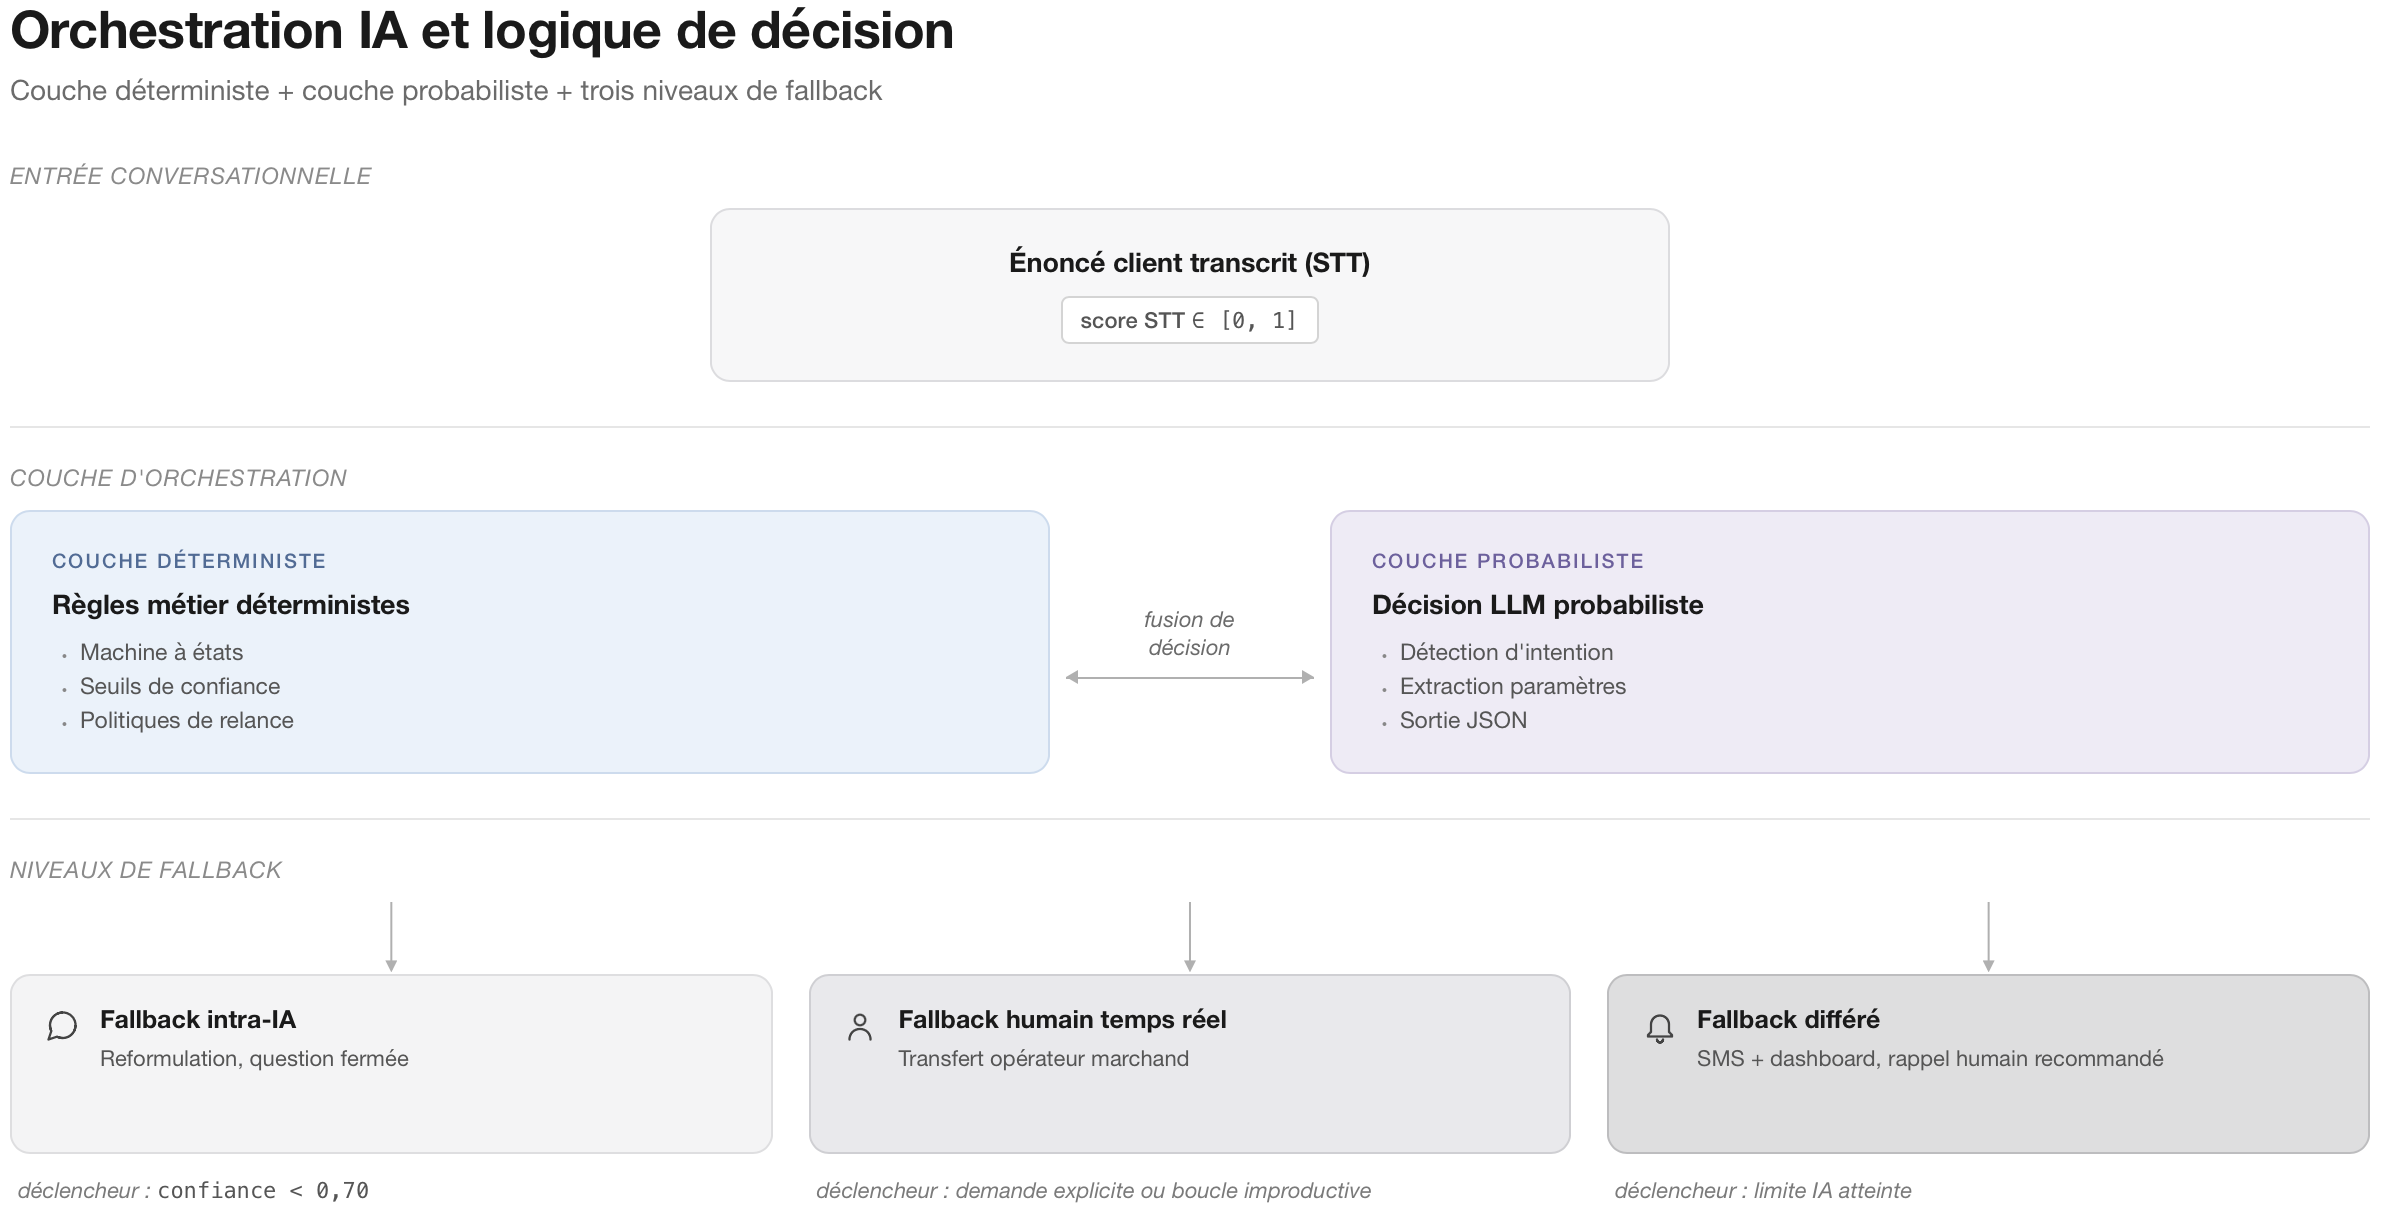
\includegraphics[width=\textwidth]{figures/orchestration_ia_vocallia.png}
\caption{Orchestration IA de Vocallia — couches de décision et niveaux de fallback}
\label{fig:orchestration_ia}
\end{figure}

\subsection{Coordination STT, LLM, TTS}
\label{subsec:orchestration_coord}

Les trois services ne sont pas appelés en série rigide mais coordonnés selon une logique adaptative. Le STT fonctionne en streaming continu, fournissant des transcriptions partielles à mesure que le client parle. Le moteur conversationnel détecte la fin d'énoncé (silence prolongé ou marqueur prosodique) et déclenche l'appel LLM. Pendant que le LLM raisonne, le moteur peut anticiper en envoyant au TTS le début d'une formule générique de transition (« \emph{matwasalsh, lehetna nchouf...} »), masquant ainsi efficacement la latence perçue. Cette technique de \emph{filler conversationnel}, courante dans les systèmes vocaux avancés, ramène la latence ressentie en deçà du seuil de gêne même lorsque la latence absolue dépasse temporairement la cible.

\subsection{Logique de décision et règles métier}
\label{subsec:orchestration_decision}

Le moteur conversationnel n'est pas un simple proxy vers le LLM. Il superpose à la décision probabiliste du modèle une couche de \textbf{règles métier déterministes} qui garantissent la prédictibilité du comportement sur les chemins critiques. À titre d'illustration~: si le LLM détecte une intention de \emph{confirmation} avec un score de confiance élevé et que le contenu de la commande lu au client a été acquitté, la commande est marquée confirmée sans nouvelle interrogation~; si le score est faible, une question de clarification fermée (« \emph{tetbet ?} » — « vous confirmez~? ») est déclenchée. Cette double couche — probabiliste pour la flexibilité linguistique, déterministe pour la rigueur métier — est la condition d'un système simultanément naturel et fiable.

\subsection{Mécanismes de fallback et escalade humaine}
\label{subsec:orchestration_fallback}

L'IA n'est pas conçue pour traiter tous les cas, mais pour traiter \emph{les cas pour lesquels elle est fiable} et pour reconnaître et escalader les autres. Trois niveaux de fallback sont implémentés. Le \textbf{premier niveau} déclenche une demande de clarification ou une reformulation lorsque la confiance STT ou LLM est trop faible. Le \textbf{deuxième niveau} transfère l'appel à un opérateur humain disponible côté marchand lorsque le client demande explicitement à parler à une personne, ou lorsque la conversation entre dans une boucle improductive. Le \textbf{troisième niveau} clôt l'appel proprement et notifie le marchand par SMS et notification dashboard, transcription à l'appui, en lui recommandant un rappel manuel. Ce dispositif à trois niveaux garantit qu'aucune commande n'est silencieusement perdue à cause d'une limitation de l'IA.

\subsection{Gestion des cas conversationnels difficiles}
\label{subsec:orchestration_edge_cases}

Cinq cas sont traités de manière explicite et systématique. Le \textbf{silence prolongé} déclenche une relance après un délai défini~; au troisième silence consécutif, l'appel est clos et marqué « indisponible — à rappeler ». L'\textbf{ambiguïté sémantique} déclenche systématiquement une question fermée disambiguante plutôt qu'un choix arbitraire. La \textbf{demande d'annulation} fait l'objet, au-delà de l'enregistrement de l'intention, d'une sollicitation optionnelle du motif (changement d'avis, prix, délai, autre), enrichissant l'analytique restituée au marchand — différenciation directe vis-à-vis des centres d'appels traditionnels. La \textbf{demande de modification de commande}, hors périmètre produit au lancement, n'est pas traitée par l'IA mais notifiée au marchand pour rappel commercial. La \textbf{demande d'information factuelle} est gérée par un \emph{knowledge base} configuré par le marchand~; toute question hors périmètre déclenche un fallback humain.

\begin{quote}
\textbf{Principe directeur de l'orchestration.} Le périmètre fonctionnel du moteur conversationnel au lancement est volontairement \emph{borné}~: il maîtrise un nombre fini de scénarios — la confirmation de commande étant le scénario d'ancrage — et reconnaît explicitement ses limites en dehors de ce périmètre. Cette discipline n'est pas une faiblesse, c'est la condition de la fiabilité. Un système qui fait peu mais le fait bien ouvre la voie à une extension progressive du périmètre, validée à chaque palier par les données opérationnelles.
\end{quote}

%%%%%%%%%%%%%%%%%%%%%%%%%%%%%%%%%%%%%%%%%%%%%%%%%%%%%%%%%%%%%%%%%%%%%%%%%%%
\section{Données, sécurité et conformité}
\label{sec:donnees_securite}
%%%%%%%%%%%%%%%%%%%%%%%%%%%%%%%%%%%%%%%%%%%%%%%%%%%%%%%%%%%%%%%%%%%%%%%%%%%

La sécurité des données et la conformité réglementaire ne sont pas des couches ajoutées en fin de conception~: elles sont des invariants architecturaux intégrés dès la conception. Cette section précise comment Vocallia traite les données qu'il manipule, comment il en protège la confidentialité et l'intégrité et comment il satisfait aux exigences légales applicables. La figure~\ref{fig:securite_donnees} en présente une vue consolidée.

\begin{figure}[H]
\centering
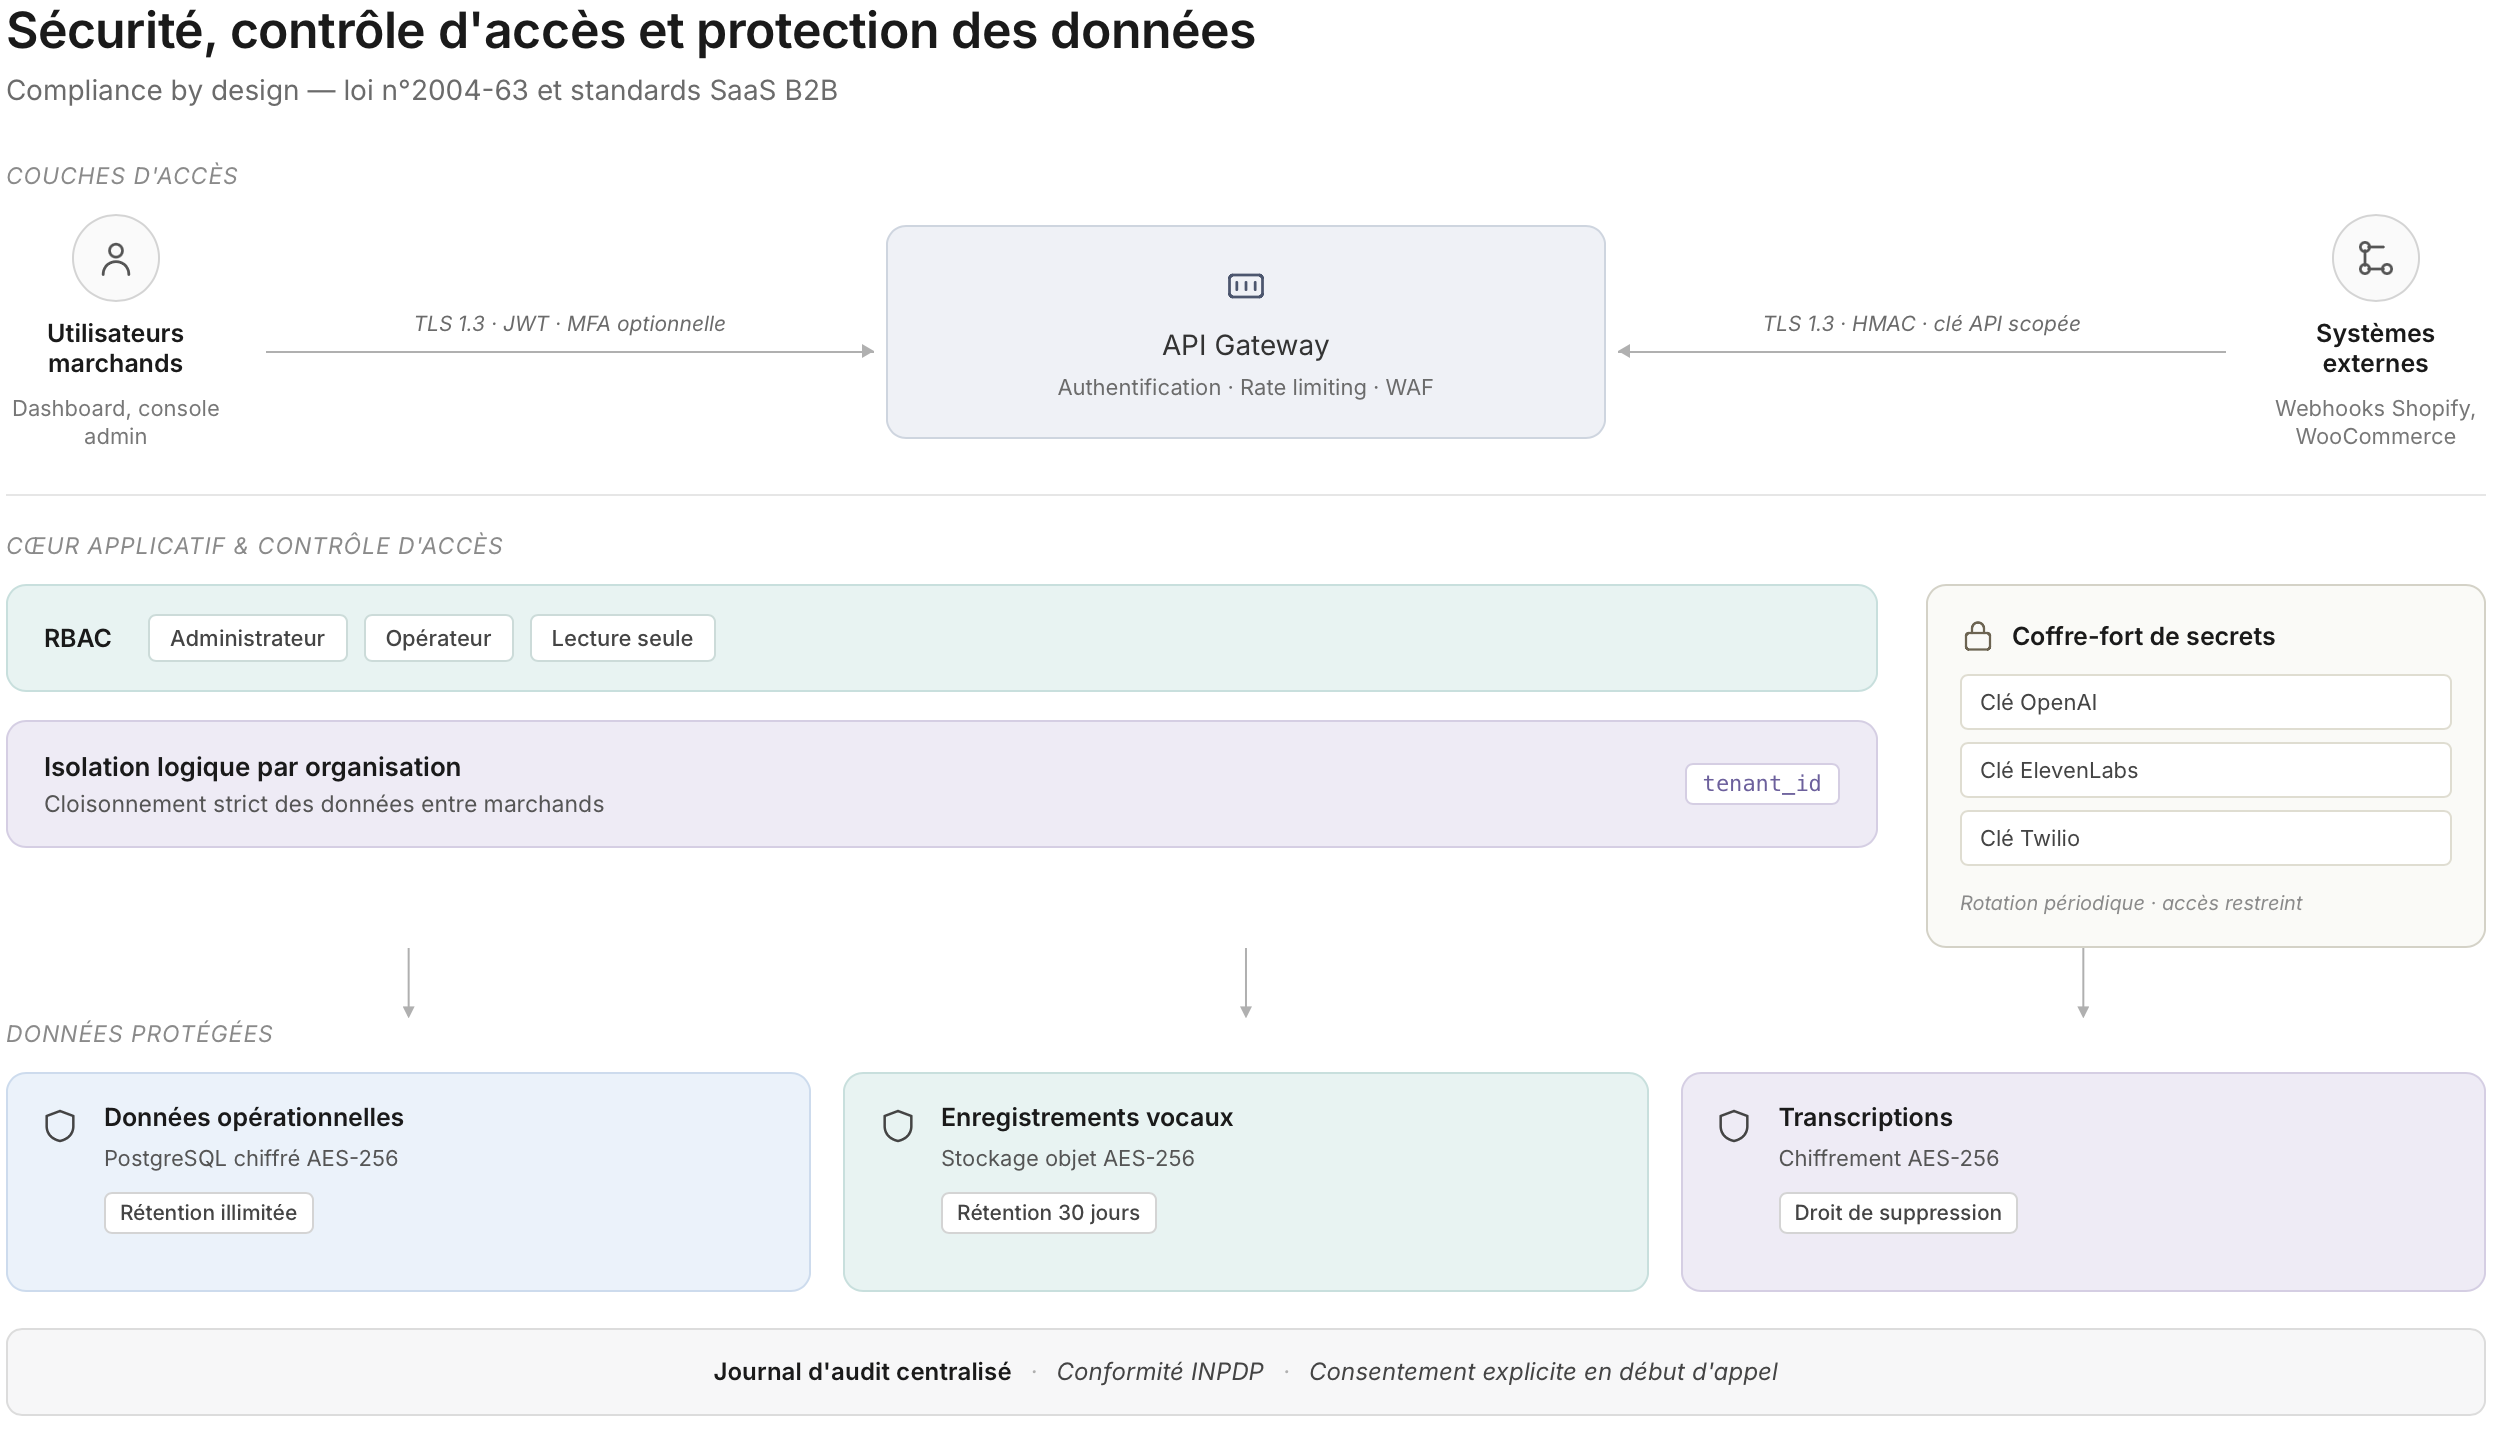
\includegraphics[width=\textwidth]{figures/securite_donnees_vocallia.png}
\caption{Architecture de sécurité et de protection des données — Vocallia}
\label{fig:securite_donnees}
\end{figure}

\subsection{Taxonomie des données manipulées}
\label{subsec:donnees_taxonomie}

Vocallia manipule cinq catégories de données, chacune soumise à des règles de traitement spécifiques. Les \textbf{données d'identité marchand} sont des données B2B classiques. Les \textbf{données opérationnelles} (commandes, statuts, métriques) appartiennent au patrimoine informationnel du marchand. Les \textbf{données personnelles des clients finaux} (numéros de téléphone, prénoms éventuels) sont les plus sensibles~: Vocallia y agit comme sous-traitant au sens de la loi n°2004-63, le marchand restant responsable du traitement. Les \textbf{enregistrements vocaux et transcriptions} constituent une catégorie particulière à laquelle la législation accorde une protection renforcée. Les \textbf{secrets techniques} (clés API, tokens, certificats) requièrent enfin une protection cryptographique systématique.

\subsection{Authentification, autorisation et isolation}
\label{subsec:donnees_authn_authz}

L'authentification des utilisateurs marchands repose sur un schéma email~/~mot de passe avec hachage robuste, complété d'une option de double authentification pour les comptes administrateur. Les sessions reposent sur des tokens JWT à durée de vie courte, accompagnés de tokens de rafraîchissement. L'authentification machine-to-machine (webhooks, API d'intégration) repose sur des clés API longues, scopées par organisation et par capacité, révocables individuellement. Au-dessus de l'authentification, un mécanisme de \textbf{contrôle d'accès basé sur les rôles} (RBAC) restreint chaque action aux rôles autorisés.

L'isolation logique entre clients constitue une exigence fondamentale d'un SaaS B2B~: aucun marchand ne doit jamais accéder aux données d'un autre. Vocallia implémente cette isolation par un pattern \emph{shared database, shared schema} avec rattachement systématique de chaque enregistrement à un identifiant d'organisation, et application de filtres au niveau de la couche d'accès aux données. Pour les comptes Pro relevant de secteurs sensibles, une option d'\textbf{isolation physique} (instance dédiée, base de données dédiée) est documentée et proposable sur devis.

\subsection{Gestion des secrets et protection des données vocales}
\label{subsec:donnees_secrets_vocal}

Les clés d'accès aux fournisseurs externes sont stockées dans un \textbf{coffre-fort de secrets} dédié (HashiCorp Vault, AWS Secrets Manager ou équivalent), jamais dans le code source ni dans des fichiers de configuration en clair. Aucune clé n'est exposée côté frontend~: tous les appels aux fournisseurs externes transitent par le backend, qui agit comme proxy sécurisé. Cette discipline élimine la classe de vulnérabilités la plus fréquente dans les architectures naïves.

Les enregistrements audio et transcriptions sont chiffrés au repos et en transit selon les standards éprouvés du secteur. Leur durée de rétention par défaut est de 30~jours, conforme à l'engagement réglementaire pris vis-à-vis de l'INPDP et explicitement annoncé aux clients finaux dans le message d'introduction d'appel. Cette rétention courte est aussi un choix d'architecture sécurité~: moins de données conservées signifie moins de surface d'attaque. Au-delà de la période de rétention, les données sont supprimées de manière irréversible. Une procédure d'effacement à la demande est prévue pour les clients finaux qui en feraient la requête via leur marchand.

\subsection{Conformité INPDP et logique réglementaire}
\label{subsec:donnees_inpdp}

La conformité à la loi n°2004-63 est intégrée par conception (\emph{compliance by design}) selon trois principes structurants. Le \textbf{consentement explicite} est obtenu en début d'appel par l'annonce de la nature automatisée et du droit du destinataire de demander un transfert humain — annonce non contournable et journalisée. La \textbf{minimisation des données} guide l'architecture~: aucune donnée sensible n'est collectée si elle n'est pas strictement nécessaire à la fonction. La \textbf{traçabilité des traitements} est assurée par un journal d'audit centralisé. Une démarche proactive d'engagement avec l'INPDP est prévue avant tout déploiement commercial à grande échelle.

\begin{quote}
\textbf{Sécurité comme avantage concurrentiel.} La rigueur sécurité et conformité décrite ici n'est pas un coût~: c'est un actif stratégique. Tout concurrent international souhaitant pénétrer le marché tunisien devra investir dans une conformité INPDP qu'il ne possède pas. Tout concurrent local moins rigoureux portera un risque juridique latent qui se matérialisera au premier contentieux. Vocallia, ayant intégré la conformité ab initio, transforme chaque renforcement réglementaire futur en avantage concurrentiel — exactement comme l'analyse PESTEL l'avait anticipé en section~2.1.
\end{quote}

%%%%%%%%%%%%%%%%%%%%%%%%%%%%%%%%%%%%%%%%%%%%%%%%%%%%%%%%%%%%%%%%%%%%%%%%%%%
\section{Scalabilité, résilience et observabilité}
\label{sec:scalabilite}
%%%%%%%%%%%%%%%%%%%%%%%%%%%%%%%%%%%%%%%%%%%%%%%%%%%%%%%%%%%%%%%%%%%%%%%%%%%

Une architecture peut être fonctionnellement correcte et néanmoins défaillir sous charge, lors de pannes externes, ou par incapacité à diagnostiquer ses propres dysfonctionnements. Trois propriétés transverses gouvernent la robustesse opérationnelle de Vocallia~: la scalabilité, la résilience et l'observabilité.

\subsection{Scalabilité de l'architecture}
\label{subsec:scal_architecture}

L'architecture de Vocallia est conçue pour scaler horizontalement, en ajoutant des instances de services plutôt qu'en augmentant la puissance d'une instance unique. Cinq choix structurels rendent ce scaling possible~: des \textbf{services applicatifs stateless}, dans lesquels aucune information de session n'est conservée localement~; une \textbf{file de messages} qui découple producteurs et consommateurs et absorbe les pics de charge~; un \textbf{cache distribué} qui réduit la pression sur la base de données~; une \textbf{séparation lecture/écriture} permettant de scaler les requêtes analytiques sans affecter les performances transactionnelles~; et un mécanisme d'\textbf{auto-scaling} qui ajuste le nombre d'instances en fonction de la charge mesurée. L'ensemble permet une montée en charge progressive cohérente avec la trajectoire commerciale projetée, sans refonte architecturale entre les paliers.

\subsection{Résilience et gestion des erreurs}
\label{subsec:scal_resilience}

La résilience de Vocallia repose sur le principe que toute dépendance externe peut défaillir, et qu'une défaillance ne doit jamais se propager en panne globale. Quatre mécanismes structurent cette résilience. Les \textbf{retries avec backoff exponentiel} sont implémentés sur tous les appels aux API externes, évitant l'effet d'avalanche en cas de saturation côté fournisseur. Les \textbf{circuit breakers} interrompent automatiquement les requêtes vers une dépendance en panne avérée, restaurant le trafic après une période de test. La \textbf{dead-letter queue} capture les jobs qui ont définitivement échoué après tous les retries, permettant leur analyse manuelle plutôt que leur perte silencieuse. Enfin, la \textbf{stratégie multi-fournisseurs} sur les couches IA et téléphonie ouvre la possibilité de basculer vers un fournisseur de secours en cas d'incident prolongé chez le fournisseur principal — exigence stratégique formalisée dans l'analyse SWOT.

\subsection{Observabilité opérationnelle}
\label{subsec:scal_observabilite}

L'observabilité repose sur les trois piliers classiques (Sridharan, 2018)~: les \textbf{logs}, les \textbf{métriques} et les \textbf{traces distribuées}. Vocallia instrumente l'ensemble de ses services pour produire ces trois types de signaux, agrégés dans une plateforme unifiée. Le tableau~\ref{tab:kpi_techniques} synthétise les principaux indicateurs surveillés en production et les actions associées en cas de dépassement.

\begin{table}[H]
\centering
\caption{Indicateurs techniques surveillés en production}
\label{tab:kpi_techniques}
\begin{tabular}{|p{5cm}|p{4cm}|p{5cm}|}
\hline
\textbf{Indicateur} & \textbf{Cible opérationnelle} & \textbf{Action en cas de dépassement} \\
\hline
Latence p95 par tour de parole & Proche de la cible & Alerte équipe technique, investigation \\
\hline
Taux d'erreur des appels API IA & Faible (<1~\%) & Bascule vers fournisseur secondaire \\
\hline
Taux d'échec de webhook entrant & Très faible & Investigation côté marchand ou Vocallia \\
\hline
Disponibilité globale du service & Élevée et continue & Post-mortem si non atteinte sur le mois \\
\hline
Taux de fallback humain involontaire & Maîtrisé & Analyse des causes, ajustement scripts \\
\hline
Score moyen de confiance STT & Élevé en moyenne & Ajustement du lexique et du \emph{prompt biasing} \\
\hline
\end{tabular}
\end{table}

Au-delà des indicateurs, des \textbf{alertes proactives} notifient l'équipe d'astreinte en cas de défaillance critique avant que les marchands n'en soient impactés. Cette posture proactive est essentielle dans un contexte SaaS B2B où chaque interruption non détectée se traduit en perte de confiance.

\begin{quote}
\textbf{Résilience face aux défaillances de fournisseurs externes.} Le scénario opérationnel le plus redouté n'est pas la défaillance interne, qu'une équipe maîtrisée peut diagnostiquer et corriger~; c'est la défaillance d'un fournisseur tiers sur lequel Vocallia n'a aucun levier direct. La réponse architecturale est triple~: substituabilité par design, dégradation gracieuse (le système continue de fonctionner avec une qualité réduite plutôt que de s'arrêter) et communication transparente vers les marchands. Cette discipline transforme un risque potentiel en simple incident géré.
\end{quote}

%%%%%%%%%%%%%%%%%%%%%%%%%%%%%%%%%%%%%%%%%%%%%%%%%%%%%%%%%%%%%%%%%%%%%%%%%%%
\section{Déploiement et exploitabilité}
\label{sec:deploiement}
%%%%%%%%%%%%%%%%%%%%%%%%%%%%%%%%%%%%%%%%%%%%%%%%%%%%%%%%%%%%%%%%%%%%%%%%%%%

Une architecture exploitable n'est pas seulement une architecture qui fonctionne~: c'est une architecture que l'on peut déployer rapidement, mettre à jour sans risque, faire évoluer sans dette accumulée et opérer avec une équipe restreinte. Ces propriétés sont particulièrement critiques pour Vocallia, dont l'équipe initiale est volontairement réduite (cf. section~3.6). La figure~\ref{fig:deploiement_monitoring} synthétise l'articulation entre pipeline de livraison, infrastructure cloud et dispositifs de résilience et d'observabilité.

\begin{figure}[H]
\centering
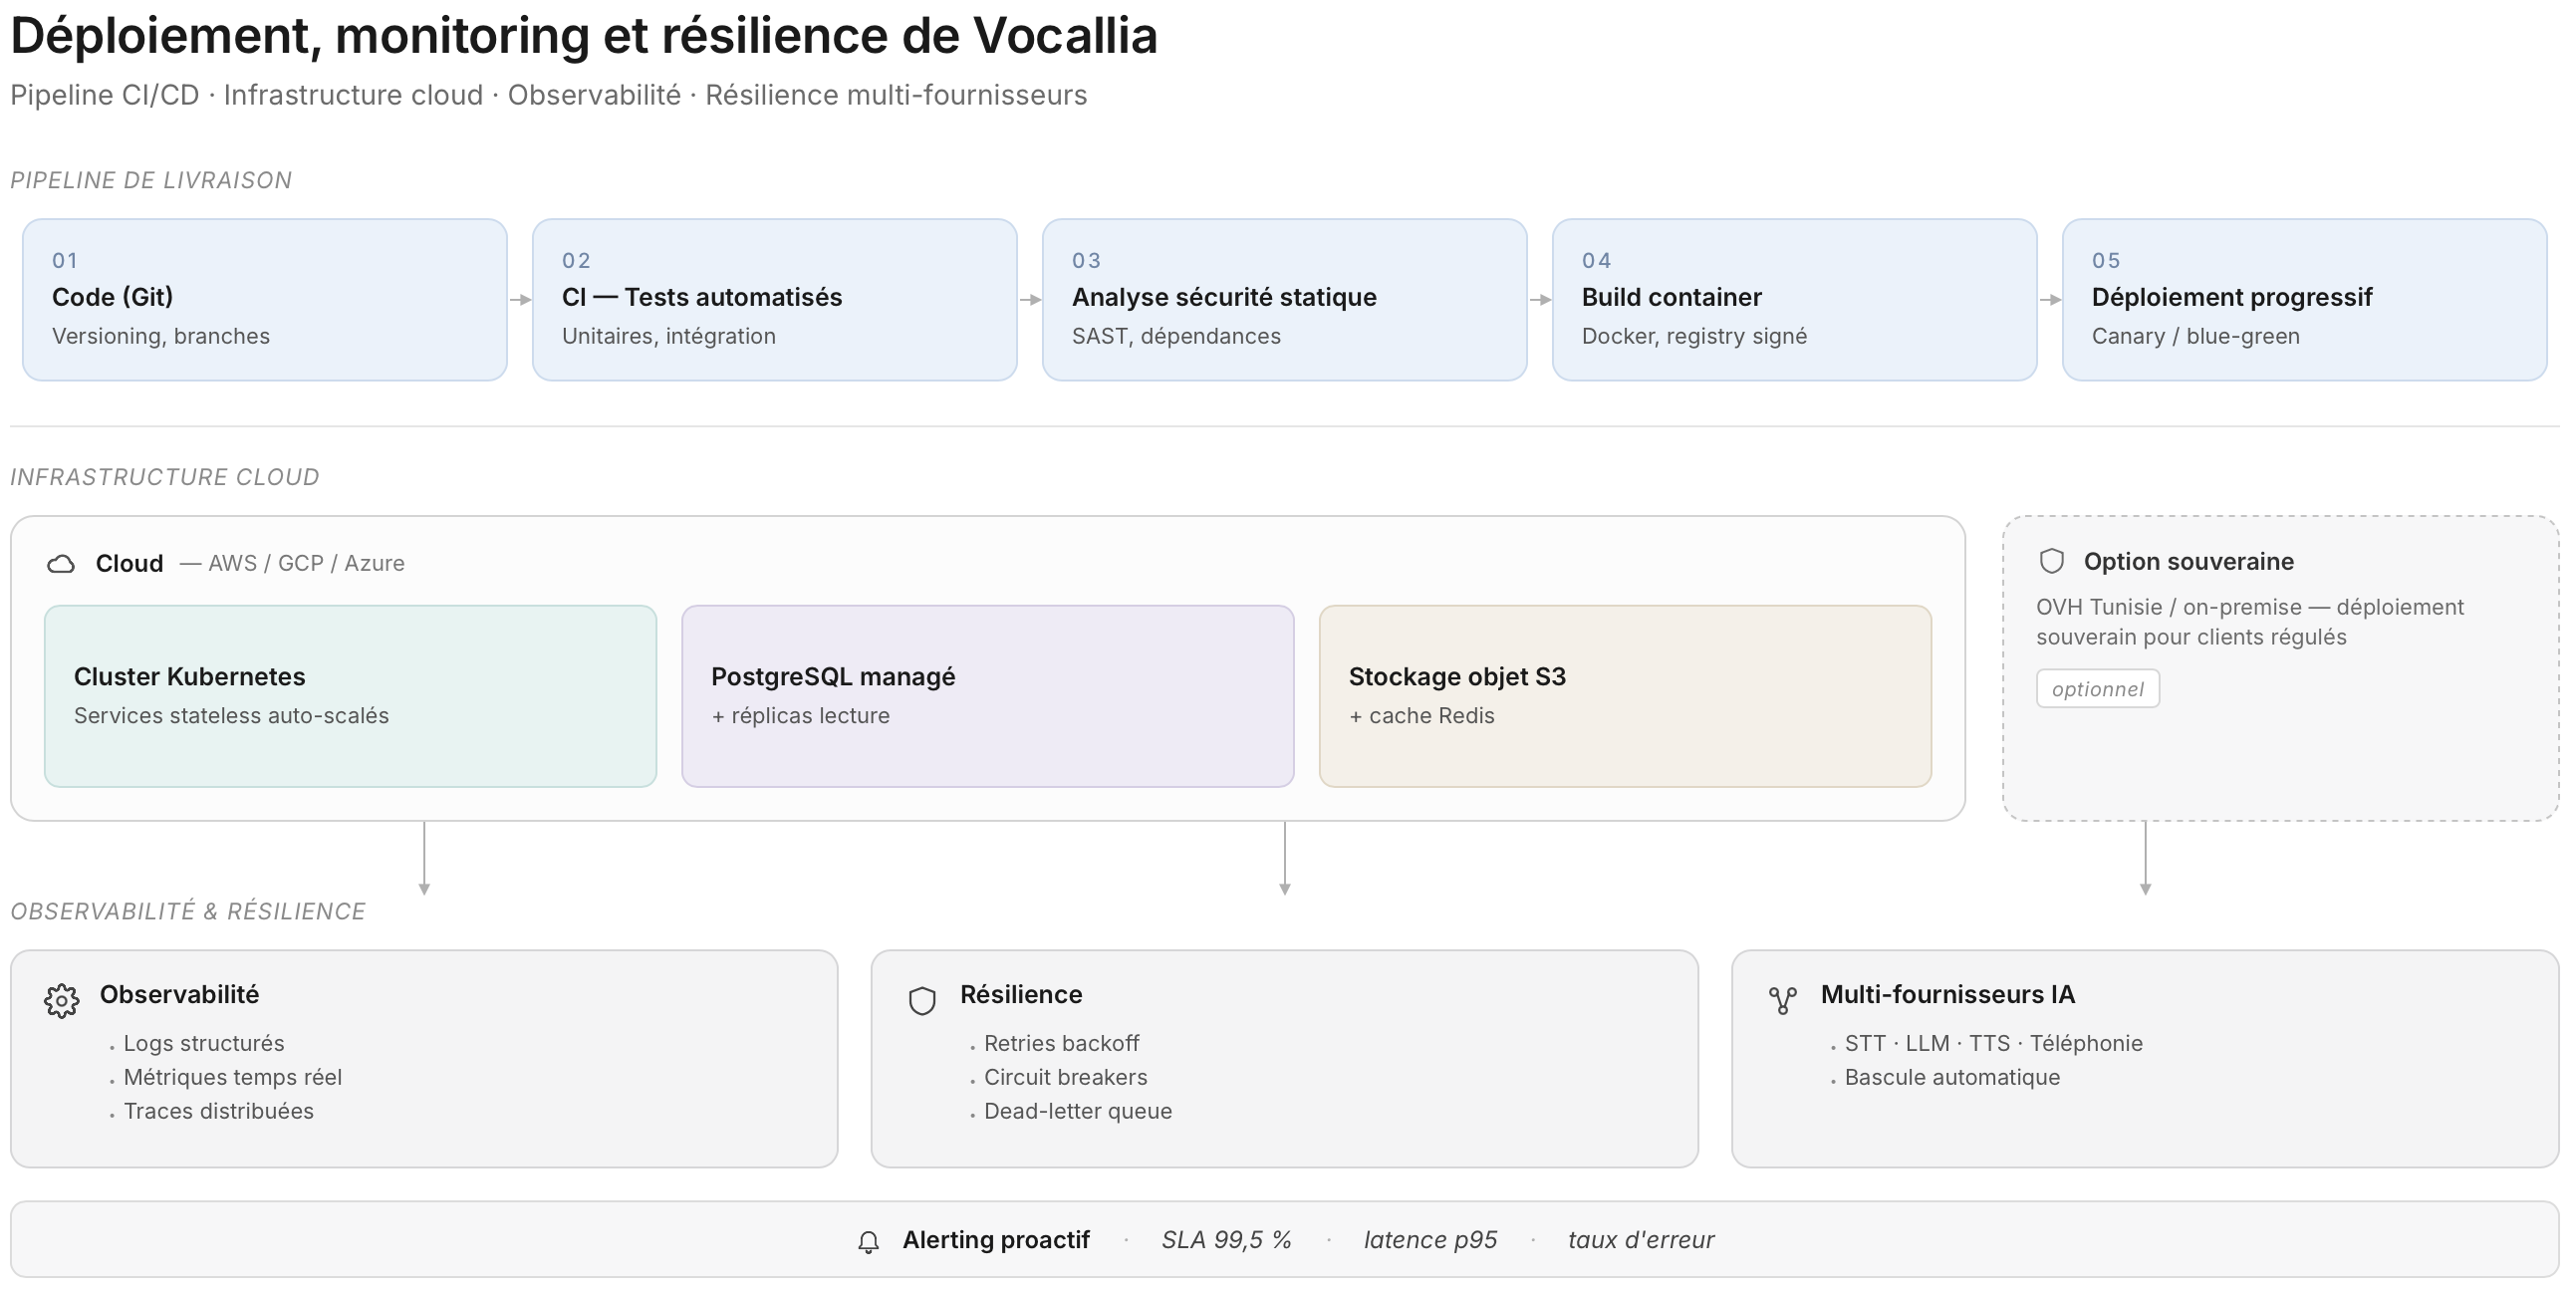
\includegraphics[width=\textwidth]{figures/deploiement_monitoring_vocallia.png}
\caption{Déploiement, monitoring et résilience de Vocallia}
\label{fig:deploiement_monitoring}
\end{figure}

\subsection{Approche cloud et infrastructure}
\label{subsec:deploiement_cloud}

Vocallia adopte une approche \emph{cloud-first} fondée sur des services managés. Le déploiement initial cible un fournisseur cloud unique (AWS, GCP ou Azure, selon les arbitrages tarifaires et de proximité régionale) avec une architecture neutre vis-à-vis du fournisseur~: l'usage de standards ouverts (Docker, Kubernetes, PostgreSQL, Redis) garantit qu'une migration future reste réalisable sans réécriture profonde. Pour les comptes institutionnels relevant de secteurs sensibles, une option de \textbf{déploiement souverain} sur infrastructure tunisienne (OVH Tunisie ou hébergement privé) est documentée. Cette option répond à la fois à des exigences éventuelles de souveraineté des données et aux préoccupations environnementales évoquées en section~2.1.

\subsection{Conditions de mise en production}
\label{subsec:deploiement_prod}

Le passage du MVP à la production opérationnelle est conditionné à une liste de critères techniques explicites~: couverture de tests automatisés sur les chemins critiques, monitoring complet déployé avec alertes configurées, procédures de \emph{runbook} documentées pour les incidents les plus probables, sauvegardes automatisées avec test de restauration validé, plan de continuité d'activité rédigé, audit de sécurité initial réalisé et procédure d'engagement INPDP initiée. Ces critères constituent une \textbf{checklist de production-readiness} dont le franchissement est une décision discrète, et non un glissement progressif.

\subsection{Maintenabilité et évolutivité}
\label{subsec:deploiement_maintenance}

Trois pratiques structurent la maintenabilité du système. L'\textbf{infrastructure as code} versionne l'ensemble de la configuration cloud, rendant les déploiements reproductibles et les modifications auditables. La \textbf{containerisation systématique} standardise les environnements de développement, de test et de production. Le \textbf{pipeline CI/CD} automatise tests, analyses statiques de qualité et de sécurité, et déploiements selon une stratégie progressive (\emph{canary} ou \emph{blue/green}) qui permet de détecter les régressions avant qu'elles n'affectent l'ensemble des marchands. L'évolutivité fonctionnelle est assurée par la modularité décrite en section~\ref{sec:architecture_logique}~: l'ajout d'un nouveau cas d'usage consiste essentiellement en l'ajout d'un scénario conversationnel et d'un connecteur d'intégration, sans toucher aux modules transverses.

\subsection{Trajectoire MVP-vers-production}
\label{subsec:deploiement_mvp}

La trajectoire technique de Vocallia s'articule en trois phases. La \textbf{phase MVP} (mois~1 à~3) délivre un système monolithique léger couvrant le scénario unique de confirmation de commande, intégré à une seule plateforme et déployé sur une infrastructure cloud minimale. La \textbf{phase pilote} (mois~3 à~6) introduit la modularisation progressive (extraction des services critiques), enrichit les intégrations, déploie le monitoring complet et engage la procédure INPDP. La \textbf{phase production} (à partir du mois~6) bascule sur l'architecture cible décrite dans le présent chapitre, avec multi-fournisseurs actifs, isolation multi-tenant durcie et observabilité complète. Cette trajectoire garantit que chaque investissement technique est calé sur un palier d'usage qui le justifie économiquement — discipline d'architecture frugale cohérente avec les contraintes de financement définies au chapitre précédent.

%%%%%%%%%%%%%%%%%%%%%%%%%%%%%%%%%%%%%%%%%%%%%%%%%%%%%%%%%%%%%%%%%%%%%%%%%%%
\section{Limites techniques et mesures de mitigation}
\label{sec:limites_mitigation}
%%%%%%%%%%%%%%%%%%%%%%%%%%%%%%%%%%%%%%%%%%%%%%%%%%%%%%%%%%%%%%%%%%%%%%%%%%%

Aucune architecture n'est sans limite. La rigueur d'un projet technique se mesure à sa capacité à identifier explicitement ses points de fragilité et à associer à chacun une mesure de mitigation crédible. Le tableau~\ref{tab:limites_mitigation} synthétise les cinq limites principales de Vocallia et la stratégie de mitigation associée.

\begin{table}[H]
\centering
\caption{Limites techniques de Vocallia et mesures de mitigation}
\label{tab:limites_mitigation}
\begin{tabular}{|p{3.5cm}|p{4.5cm}|p{6cm}|}
\hline
\textbf{Limite} & \textbf{Nature du risque} & \textbf{Mesures de mitigation} \\
\hline
Variabilité dialectale & Variations régionales et générationnelles du darija mal couvertes par les modèles génériques & \emph{Prompt biasing} avec lexique tunisien~; constitution d'un corpus propriétaire à partir des appels traités~; cycle d'amélioration mensuel des scripts~; fallback humain en cas de confiance faible \\
\hline
Latence cumulée & Le pipeline STT~$\to$~LLM~$\to$~TTS peut dépasser ponctuellement la cible de latence & Streaming bout en bout~; mise en cache des introductions vocales~; \emph{filler conversationnels} masquant la latence~; surveillance p95 et alerting \\
\hline
Dépendance fournisseurs tiers & Hausse tarifaire, interruption de service ou changement de CGU des API externes & Architecture multi-fournisseurs avec adaptateurs interchangeables~; circuit breakers~; possibilité de bascule vers fournisseur secondaire \\
\hline
Fiabilité de la téléphonie sortante & Échec de connexion, qualité audio dégradée, blocage par opérateurs anti-spam & Stratégie de retry sur appels échoués~; surveillance des taux par opérateur destinataire~; partenariat futur potentiel avec opérateur local \\
\hline
Volatilité des prix d'API IA & Modification des tarifs OpenAI / ElevenLabs impactant la marge brute & Veille tarifaire continue~; possibilité de bascule vers alternatives (Claude, Mistral, Coqui)~; économies d'échelle avec la croissance du volume \\
\hline
\end{tabular}
\end{table}

Au-delà du tableau, deux principes transverses gouvernent la posture de Vocallia face à ces limites. Le premier est la \textbf{transparence assumée}~: aucune limite n'est dissimulée aux marchands. Lorsqu'une interaction sort du périmètre de fiabilité de l'IA, le marchand est notifié et le rappel humain est explicitement recommandé. Cette transparence préserve efficacement la confiance, bien plus qu'une promesse universelle qui se révélerait fausse. Le second est la \textbf{conversion progressive des limites en avantages compétitifs}~: chaque appel traité enrichit le corpus dialectal propriétaire de Vocallia. Ce qui constitue aujourd'hui une limite — couverture imparfaite des sous-registres dialectaux — devient demain un actif que les concurrents entrants ne pourront pas répliquer instantanément, exactement le mécanisme de \emph{flywheel} décrit en figure~2.9 du chapitre~2.

\begin{quote}
\textbf{Discipline face aux limites.} La force d'une architecture ne réside pas dans l'absence de limites — qui serait illusoire — mais dans le fait que chaque limite est identifiée explicitement, surveillée techniquement, mitigée concrètement et inscrite dans une dynamique d'amélioration mesurable. Aucune des cinq limites ci-dessus n'est rédhibitoire pour le lancement~; toutes sont instrumentées et adressées par une mesure de mitigation directement opérationnelle.
\end{quote}

%%%%%%%%%%%%%%%%%%%%%%%%%%%%%%%%%%%%%%%%%%%%%%%%%%%%%%%%%%%%%%%%%%%%%%%%%%%
\section{Conclusion}
\label{sec:conclusion_chap4}
%%%%%%%%%%%%%%%%%%%%%%%%%%%%%%%%%%%%%%%%%%%%%%%%%%%%%%%%%%%%%%%%%%%%%%%%%%%

L'analyse technique conduite dans ce chapitre établit quatre conclusions qui valident la viabilité technique de Vocallia.

\textbf{La solution est techniquement réalisable avec les technologies actuelles.} Chacun des composants du pipeline conversationnel — reconnaissance vocale, modèle de langage, synthèse vocale, téléphonie programmable — est aujourd'hui disponible en mode service à des conditions économiques compatibles avec le pricing défini en section~3.8. Le coût variable par appel de deux minutes, estimé autour de 0{,}27~DT, est cohérent avec un prix d'entrée Starter de 0{,}79~DT par appel et préserve une marge brute soutenable de l'ordre de 65~\%. La latence cible reste atteignable grâce au streaming et à une orchestration soignée, et la couverture dialectale est suffisante au lancement avec les mécanismes de mitigation mis en place.

\textbf{L'architecture est cohérente avec les objectifs produit.} La modularité en sept blocs métier traduit directement la roadmap d'extension multi-cas d'usage. La séparation en cinq couches techniques garantit l'évolutivité, la testabilité et la substituabilité des fournisseurs. La conception multi-tenant et la conformité INPDP intégrée ab initio sont les conditions techniques de la promesse commerciale formulée aux marchands. Aucune décision technique n'est gratuite~: chacune découle d'une exigence produit ou d'une contrainte explicitement identifiée.

\textbf{Les risques techniques sont identifiés, surveillés et adressés.} Les cinq limites principales — variabilité dialectale, latence, dépendance fournisseurs, fiabilité téléphonique, volatilité tarifaire — sont chacune associées à une mesure de mitigation opérationnelle. La résilience est assurée par la redondance multi-fournisseurs, les retries, les circuit breakers et la dégradation gracieuse. L'observabilité complète permet le diagnostic rapide et l'amélioration continue. Aucun risque technique identifié ne constitue un obstacle rédhibitoire au lancement.

\textbf{L'architecture est évolutive, pas figée.} La trajectoire MVP~$\to$~pilote~$\to$~production permet de calibrer chaque investissement technique sur le palier d'usage qui le justifie. La modularité interne autorise l'ajout de nouveaux cas d'usage sans refonte. L'option de déploiement souverain ouvre l'accès aux secteurs institutionnels sensibles. Le système est conçu pour grandir avec Vocallia, pas pour être réécrit à chaque palier.

L'ensemble de ces éléments converge vers une conclusion sans ambiguïté~: \emph{Vocallia est techniquement viable}. L'architecture proposée n'est ni surdimensionnée pour le lancement ni sous-dimensionnée pour la croissance~; elle est calibrée sur la trajectoire commerciale projetée au chapitre précédent, et conçue pour servir la promesse produit définie au chapitre~3, dans les contraintes de marché établies au chapitre~2.

Le chapitre suivant prolonge cette analyse sur le terrain de la viabilité financière et de l'exécution opérationnelle~: budget initial, plan de financement, chronogramme de lancement, jalons critiques, et conditions de transformation de la solution technique en activité économique pérenne.